\section{Sequence labelling}

Word order is crucial for understanding the meaning of text and for tasks like classification. 
While $n$-grams can help capture word order, they are inherently limited in length and may fail to fully represent complex dependencies.

\begin{definition}[\textit{Sequence classification}]
    Sequence classification takes an ordered sequence of tokens as input and produces a single prediction for the entire sequence.
\end{definition}

\begin{definition}[\textit{Sequence labelling}]
    Sequence labeling takes an ordered sequence of tokens as input and generates a corresponding sequence of predictions.
\end{definition}

Historically, sequence labeling has been tackled using:
\begin{itemize}
    \item \textit{Hidden Markov Models}: these function similarly to Naïve Bayes but applied to sequences. 
        An Hidden Markov Model consists of: hidden states (unobserved), observed words (the actual text), transition probabilities (likelihood of moving between hidden states), and emission probabilities (likelihood of words appearing in specific states).
        Parameter estimation is typically done by counting frequencies in labeled data. 
        If hidden states are unknown, the Expectation-Maximization algorithm can be used.
    \item \textit{Conditional Random Fields}: these operate similarly to Logistic Regression but for sequential data. 
        Instead of using transition and emission probabilities like Hidden Markov Models, Conditional Random Fields employ undirected potentials:
        \begin{itemize}
            \item $\phi(t_1,t_2)$ for transitions between labels. 
            \item $\phi(t_1,w_1)$ for label-word relationships.
        \end{itemize}
        By relaxing the generative assumption, Conditional Random Fields often achieve better performance while keeping parameter estimation similar.
\end{itemize}
\noindent Recent advancements leverage Recurrent Neural Networks to further improve sequence labeling performance by capturing long-range dependencies more effectively.

\subsection{Recurrent Neural Networks}
Word embeddings represent words in a continuous semantic space. 
To aggregate embeddings and represent an entire document, one approach is to sum them, similar to how one-hot encodings create a bag-of-words representation. 
However, this method ignores word order, leading to documents with different structures but similar words having the same representation.

Recurrent Neural Networks provide a more effective way to accumulate information across a document while preserving word order. 
They achieve this by sequentially combining the embedding of the current word with the context from previous words.

Recurrent Neural Networks operate using a simple yet powerful structure. 
They take two vectors as input: the current input and the previous state. 
They then produce two vectors as output: the current output and the updated state. 
This structure allows Recurrent Neural Networks to process arbitrarily long input sequences and encode them into a single embedding.

\subsection{Long Short-Term Memory}
Long Short-Term Memory (LSTM) is an advanced variant of RNNs designed to learn context and capture long-range dependencies. 
It achieves this through a gating mechanism that controls the flow of information:
\begin{itemize}
    \item Information passes through by default unless explicitly modified.
    \item New information can be added to the state.
    \item Irrelevant information can be removed (forgotten).
\end{itemize}
\noindent LSTMs learn when to remember, forget, and output information at each timestep, making them highly effective for sequential data.
\begin{figure}[H]
    \centering
    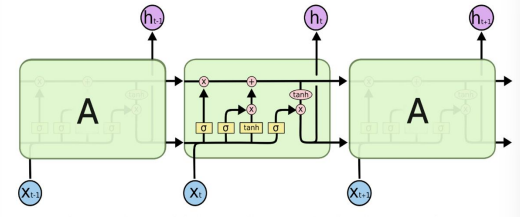
\includegraphics[width=0.5\linewidth]{images/nlp1.png}
    \caption{Long Short-Term Memory}
\end{figure}
LSTMs can be stacked to form deeper networks, enhancing their ability to handle nested contexts. 
This capability is particularly useful for processing natural language, where understanding hierarchical structures and long-term dependencies is essential.

\subsection{Applications}
Sequence classifiers and sequence labelers are widely used in various NLP tasks.

\paragraph*{Part of Speech tagging}
Modern grammar categorizes words into open and closed classes.
\begin{figure}[H]
    \centering
    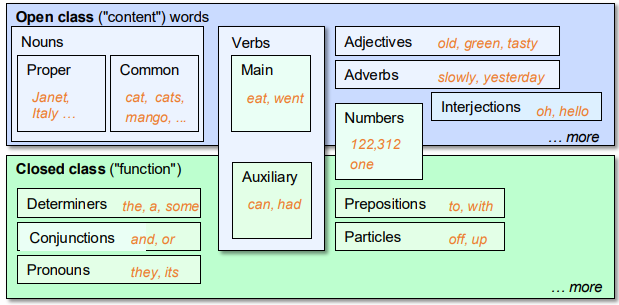
\includegraphics[width=0.5\linewidth]{images/nlp2.png}
    \caption{Modern grammar}
\end{figure}
POS tagging involves assigning a part-of-speech label to each token in a sequence. 
This is useful for:
\begin{itemize}
    \item Developing features for NLP models.
    \item Reducing ambiguity in bag-of-words representations by appending POS tags to word occurrences.
    \item Serving as a foundational step for other NLP tasks, such as syntactic parsing and linguistic analysis.
    \item Supporting applications like text-to-speech and the study of linguistic chang.
\end{itemize}
\noindent POS tagging maps a sequence of words $(x_1,\dots,x_n)$ to a sequence of POS tags $(y_1,\dots,y_n)$
Although 85\% of English vocabulary terms are unambiguous, about 60\% of tokens in actual text are ambiguous, making POS tagging a challenging task. 
However, modern systems achieve an accuracy of around 97\%, which is comparable to human performance.

\paragraph*{Named Entity Recognition}
Named Entity Recognition is the task of identifying entities mentioned in a text. 
It is typically framed as a sequence labeling problem and serves as a crucial step in extracting structured knowledge from unstructured text.

A named entity refers to an object in the real world. 
Common entity categories include: PER (person), LOC (location), ORG (organization), GPE (geo-political entity). 
Entities are often multi-word phrases, and the term named entity has been extended to cover concepts beyond just real-world objects.

Named Entity Recognition involves two key steps identify spans of text that represent proper names and assign a label that categorizes the type of entity.

Traditional Applications of Named Entity Recognition includes: 
\begin{itemize}
    \item \textit{Sentiment analysis}: detecting sentiment toward something.
    \item \textit{Information extraction}: extracting structured facts about entities from raw text.
    \item \textit{Question answering}: understanding entity-related questions and retrieving relevant information.
    \item \textit{De-identification}: removing personal references from text to ensure privacy.
\end{itemize}
\noindent The main challenges in Named Entity Recognition are: 
\begin{enumerate}
    \item \textit{Segmentation}: unlike POS tagging, where each word has a single tag, named entities can span multiple words.
    \item \textit{Type ambiguity}: the same word or phrase can have different meanings depending on context.
\end{enumerate}
\noindent To transform NER into a sequence labeling task (assigning one label per token), the Begin-Inside-Outside (BIO) tagging scheme is commonly used:
\begin{itemize}
    \item \textit{Begin} (B): the first token in an entity span.
    \item \textit{Inside} (I): tokens inside the entity span.
    \item \textit{Outside} (O): tokens that do not belong to any entity.
\end{itemize}
\noindent This approach enables models to correctly identify and classify multi-word entities within a text.

\paragraph*{Entity Linkage}
Identifying a named entity in text is only the first step. 
The next challenge is determining which real-world entity the mention refers to, a process known as entity linkage.
This task is difficult due to ambiguity. 

Entity linkage methods rely on the relative importance of entities and context within the text, including other mentioned entities that provide clues.

Entity linkage typically uses structured knowledge sources. 
However, many individuals or objects lack a source. 
In such cases, custom ontologies are used for better accuracy.

\paragraph*{Relation extraction}
Once entity mentions are correctly linked to real-world entities, the next step is relation extraction—identifying relationships between entities to build structured knowledge.
Extracted relationships can be used to populate a knowledge graph or knowledge base.
This is often framed as a problem of predicting missing links in a graph.
Entity embeddings help model relationships, as spatial transformations in embedding space naturally encode relational patterns.

\subsection{Parse trees}
Parse trees (also called syntax parse trees or dependency parse trees) represent the structure of a sentence based on a formal grammar. 
These grammars define a set of rules for generating valid text and are commonly used for analyzing both natural language and programming languages.
Given a piece of text, parsing reverses the generative process by identifying which grammatical rules were applied and the order in which they were applied
This recursive process results in a tree structure for each sentence, where each node represents a syntactic component.

Parse trees help determine how words in a sentence relate to one another. 
This structural analysis allows us to infer the intended meaning (semantics) of the sentence.

In theory, formal grammars alone could be used to parse text.
However, natural language is inherently ambiguous, and formal grammars tend to be brittle (struggling with variations in phrasing). 
In practice, machine learning techniques are often needed to extract accurate parse trees from real-world text.

Understanding sentence structure is crucial for many NLP tasks, including: populating structured databases, generating coherent text, and extracting relationships

\subsection{Co-reference, taxonomy and ontology}
\begin{definition}[\textit{Co-reference}]
    Co-reference resolution is the task of determining who or what a given pronoun or noun phrase refers to within or across sentences.
\end{definition}
\noindent In most cases, a pronoun appears after its referent in the text.
However, there are instances where the pronoun appears before the referent, requiring more complex resolution strategies.

It helps in understanding what is being said about an entity, especially when pronouns are used.
It is crucial for tasks such as information extraction, chatbots, and text summarization, where accurate entity tracking is needed.

\begin{definition}[\textit{Taxonomy}]
    Taxonomy is the hierarchical structure of concepts. 
\end{definition}
\begin{definition}[\textit{Ontology}]
    Ontology is the formal representation of concepts and their relationships.
\end{definition}
Ontologies typically consist of the following components: classes, individual, attributes, relationships, and logical rules. 

In an ontology or knowledge base, the relationships between concepts form a graph structure. 
These knowledge representations capture the factual information conveyed in sentences, enabling better comprehension and reasoning.

Ontologies and knowledge bases typically follow open world semantics, where any statement not known to be true is simply unknown. 
This contrasts with the closed world assumption used in databases, where any statement not known to be true is assumed false.